\documentclass[a4paper,10pt]{article}

\usepackage[utf8]{inputenc}
\usepackage{graphicx}
\usepackage{mathtools}

\title{SDSS Celestial Objects Classification}
\author{Andrea Sessa \\ \vspace{1cm} \small{Mat. 850082}}
\date{}

\begin{document}

\maketitle

\begin{abstract}
  The project aims to study the problem of dimensionality reduction in the field of astronomy.
  The high number of features involved often makes the job of classifying celestial objects, 
  basing entirely on their spectra, very difficult. The problem of preprocessing high dimensional 
  astronomical data is considered. We refer to the method described in \cite{redshift} to 
  overcome the problem of missing data and the different redshift factor of different object.
  The resulting dataset(which is the starting point for the project) contains information of
  4000 celestial object(such as galaxies, quasars, stars, etc.) each of the samples consists
  of 1000 attributes which describe the electromagnetic radiation over different wavelength(3000 to 8000 angstrom).
  We propose different methodologies to approach the problem of features reduction:
  PCA, Kernel PCA(different kernel are considered) and forward/backward features selection;
  The goodness of each method is evaluated over Support Vector Machine(soft margin penalty is tuned by 5-Fold cross-validation)
  considering as metrics accuracy, precision, recall and F1 score.
  Final results shows, in general, how a very small number of features in the can actually capture an high percentage(90 \%)
  of the variance associated with the data.
\end{abstract}

\newpage

\tableofcontents

\newpage

\listoffigures

\newpage

\section{Introduction}
  Modern astronomy is concerned with the study of very distant celestial objects ie quasars, galaxies, stars, etc.\newline
  Often this type of classification is performed by analyzing the spectrum emitted by such objects.\newline
  In general the emission spectrum of a chemical element or of a chemical compound is defined as the electromagnetic radiation emitted
  when an atom or a molecule, of the object that we are observing, perform a transition from an high energy states to a low energy state.
  During the decadiment the atom or molecule the electromagnetic is irradiated under the form of photon, the associated photon energy
  (also called flux) is proportional is equal to the energy difference between the two energy states involved in the decadiment.\newline
  The important element is that for a given atom there are many possible electron transition, and each of these transition has a specific
  flux associated.\newline
  The Sloan Digital Sky Survey(henceforth referred as SDSS) is a major imaging and spectroscopic survey using a dedicated 2.5-m wide-angle
  optical telescope at Apache Point Observatory in New Mexico, United States.\newline
  The collection of data started in 2000 and continues up to nowadays(latest data release in June 2013). The dataset comprises almost
  2 millions of spectra coming from different objects.\newline
  Machine learning plays an important role in the task of classifying these objects, given the fact that many times samples include
  more than 1000 features.\newline
  Features in general includes information about the flux associated with a specific wavelength.
  
  \begin{figure}[!ht]
    \caption{Typical emission spectrum for an emission galaxy}
    \centering
    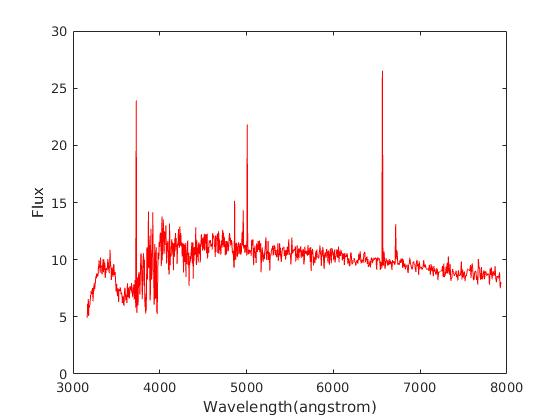
\includegraphics[scale=0.5]{emission_galaxy.jpg}
  \end{figure}
  
  If the input feature vectors have very high dimension, the learning problem can be difficult even if the true function only depends on a small number of those features.
  This is because the many "extra" dimensions can confuse the learning algorithm and cause it to have high variance.
  Hence the problem of features selection become very important in this scenario; this project will try to cast
  some light on the problem by evaluating different approaches over a reduced version of the SDSS dataset.
  
\section{Problem Formulation}
  The overall problem is divided into three main sections:
  \subsubsection{Features Extraction}
  The first one is the issue of features selection, what follows is a possible formal formulation of the problem:\newline
  The goal is, starting from a number of features $ M = 1000 $, find $M' \ll M$ such that 
  the selected $M'$ features gives the smallest expected generalization error. In more formal terms:\newline\newline
  
  \textit{Given a set of functions $y = f(x,\alpha)$ we want to find a preprocessing over the data, $\textbf{x} \mapsto (\textbf{x} * \sigma)$}
  \begin{equation}
    \tau(\sigma, \alpha) = \int \mathrm V(y,f((x*\sigma),\alpha) \,\mathrm{d}p(\textbf{x},y)
  \end{equation}
  \textit{subject to $||\sigma||_0 = M'$,  where $p(x,y)$ is unknown, $x * \sigma = (x_1 \sigma_1, ... , x_M \sigma_M)$ denotes an
  element wise product, $V (.,.)$ is a generic loss function} \newline
  The literature divided the feautures selected methods into two main group
  \begin{itemize}
   \item \textbf{Filter methods} rely on general characteristics of the data to evaluate and to select the feature subsets without
	 involving the chosen learning algorithm. Scores are assigned to each features according to some metrics.\newline
	 A widely-used filter method is to apply a classical univariate ANOVA F-Test. The procedure
	 calculates the following F-statistics for each feature:\newline\newline
	 \textit{Y = generic label(0 to 9) \newline $N_j$ = number of samples with Y = j \newline $\bar{x}_j$ = the sample mean for features X for target class j
		 \newline $s_{j}^2 = \sum_{i=1}^{N_j} (x_{ij} - \bar{x}_j) / (N_j -1)$ 
		 \newline $\bar{x} = \sum_{j=1}^{J} N_j\bar{x}_j / N$ }\newline
	 \begin{equation}
	  F = \frac{\sum_{j=1}^{J} N_j(\bar{x}_j - \bar{x})^2 / (J - 1)}{\sum_{j=1}^{J} (N_j - 1)s_{j}^2 / N_j -1} \sim F(J-1, N-J)
	 \end{equation}
	 If the null hypothesis is accepted then the feature X is statistically significant for the classification.\newline 
	 From the statistics we can assign a p-value to each features and rank them(ascending order); if the p-value is smaller
	 than the significant level than the test accept the null hypothesis.\newline

   \item \textbf{Wrapper methods} evaluate subsets of features which allows, unlike filter approaches, to detect the possible
	 interactions between features.\newline
	 Sequential feature selection is one of the most widely used techniques. It selects a subset of features by sequentially adding 
	 (forward search) or removing (backward search) until certain stopping conditions are satisfied.
	 For this project we will consider a forward search, the algorithm stops when a local minima is obeserved in the metric used
	 to evaluate the goodness of the subset.
  \end{itemize}
  
  \subsubsection{Dimensionality Reduction}
    The objective of dimensionality reduction differs from the idea behind features selection, while the latter tries to select
    the best subset, a dimensionality reduction algorithm applies a transformation over the existing features re-projecting the 
    data over a dimensionality reduced dataset.\newline
    In more formal terms, we are trying to find a orthogonal transformation matrix $W$ such that:
    \begin{equation}
     \overline{X} = W^T X
    \end{equation}
    $\overline{X}$ is new dimensionality rappresentation of the data.
  
  \subsubsection{Classification - Multi-class SVM}
     Support Vector Machines (henceforth referred as SVM) are supervised learning models with associated learning algorithms
     that analyze data used for classification (and regression).\newline
     We focus our attention first on the case of binary classification and the we extend it to the general case of multi-class classification.\newline
     In a two-class SVM the prediction for a new point is given by:
     \begin{equation}
      f(x_q) = sign \left( \sum_{m \in M} \alpha_m t_m k(x_q, x_m) + b \right ) 
     \end{equation}
     The objective of a SVM is to maximize the margin that is the distance of the closest point to the separating hyperplane.
     The problem maximize the margin leads to the following constrained optimization problem:
     \begin{equation}
      \begin{aligned}
	& \underset{x}{\text{min}}
	& & \frac{1}{2} ||w||_2^2 + C \sum_{i} \xi_i  \\
	& \text{subject to}
	& & t_i(w^T x_i + b) \geq 1 - \xi_i \; \forall i
      \end{aligned}
     \end{equation}
     The previous equation permits to assign to each sample a weight($\alpha$) that determine the so-called support vector.\newline
     However in our case the problem must be formulated in terms of a generic number of classes($K=7$ classes).\newline
     Different approaches to the problem, for this project we follow a \textit{1 versus 1} approach: for each pairs of classes
     we solve a binary SVM classification problem as described above. The number of pair to be considered is given by
     \begin{equation}
      \textrm{N of comparisons} = \frac{K(K-1)}{2}
     \end{equation}
     A comparison with others possible approach \cite{multisvm}, eg \textit{1 versus the rest}, shows that \textit{1 versus 1}
     in general has good performance(very short training time) but in some cases it can lead to situations in which samples are
     ambiguously classified.

\section{Methodology}
  In this section is included a list(and a brief description) of the approaches that will be considered during the experimentation campaign.\newline
  Details and experimentation results are given is section 4.
  
  \subsection{Baseline Classifier}
    The baseline is represented by a standard 7-class SVM classifier, all the dataset is used, no features selection/dimensionality
    reduction algorithm is applied. The SVM uses a gaussian kernel defined has:
    \begin{equation}
     k(x,y) = exp \left( \frac{-||x-y||^2}{2 \gamma} \right)
    \end{equation}
    The hyperparameter $\gamma$(the `spread` of the gaussian curve) and $C$ (the penalty for miss-classified point) are chosen by 5-fold
    cross validation iterating over a grid of possible value.
  
  \subsection{ANOVA F-Test}
    

\section{Experiments}
  \subsection{Dataset Description}
    The dataset that has been used for this project is a reduced version of the SDSS spectroscopic dataset:
    it consisted of 4000 spectroscopic samples, each of this sample formed by 1000 features that describes 
    the spectrum over the different wavelength.\newline
    Objects in the dataset belong to 7 different categories:
    \begin{enumerate}
      \item \textbf{STAR}: Generic stellar objects
      \item \textbf{ABSORPTION GALAXY}: Galaxies that show relatively homogeneous spectra, dominated by absorption features from cool giant stars
      \item \textbf{GALAXY}: Generic galaxy(neither absorption nor emission)
      \item \textbf{EMISSION GALAXY}: Galaxies whose spectrum is dominated by emission features
      \item \textbf{NARROW-LINE QSO}: Narrow emission quasars
      \item \textbf{BROAD-LINE QSO}: Broad emission quasars
      \item \textbf{LATE-TYPE STAR}: Cooled starts(type K or type M)
    \end{enumerate}
  
  \subsubsection{Preprocessing}
    This project do not use the original SDSS dataset(which contained more than 4000 features per sample!).\newline
    The samples present in the original dataset had two main problems:
    \begin{itemize}
     \item Each individual spectra present a different redshift factor(z). This phenomena is due to the fact that 
	the object that was being observed, was moving during while emitting light, this cause the frequency of light
	to `shift` toward lower energy wavelength ie. toward `red`.
     
     \item Missing data: There are several reasons for gaps to exist: The removal of skylines,
	bad pixels on the CCD chips all leave gaps at different frame wavelengths for each spectrum, general technical problem, etc. 
	All these factor can contribute to incomplete spectra.\newline
	To overcome this problem a Principal Component Analysis(henceforth referred as PCA) is used to reproject the data
	on their principal dimension and then used to fill the missing gap. The entire procedure is described in detail in \cite{redshift}
    \end{itemize}
    In addition to the two above stated procedure the dataset has been further downsampled till to reduce the number of significant features
    to 1000(which is still quite high!).\newline
    Finally, given the fact that the spectra belong to very different celestial object at very different distance(light years order) from 
    the observation point, a final step of normalization is applied that is Z-Score and mean centering(making them suitable for a subsequent PCA analysis).
  
  \subsubsection{Visualization}
    In figure 2 are shown some random spectra for different type of objected extracted from the dataset:
    
    \begin{figure}[!ht]
      \caption{Sample spectrum for different objects}
      \centering
      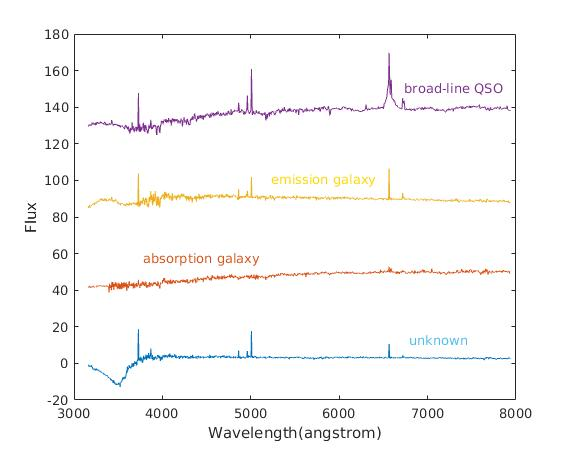
\includegraphics[scale=0.6]{sample_spec.jpg}
    \end{figure}

\section{Conclusions}

\begin{thebibliography}{9}
  \bibitem{spectrum}
    Wikipedia,
    \emph{Emission Spectrum}
    
   \bibitem{sdss}
    Wikipedia,
    \emph{The Sloan Digital Sky Survey}
    
   \bibitem{redshift}
    C.W. Yip et al,
    \emph{Spectral Classification of Quasars in the Sloan Digital Sky Survey: Eigenspectra, Redshift, and Luminosity Effects},
    Astronomical Journal,
    2004
    
    \bibitem{multisvm}
     Chih-Wei Hsu, Chih-Jen Lin
     \emph{A Comparison of Methods for Multi-class Support Vector Machines},
     IEEE Transactions on Neural Networks, 13(2002), 415-425
\end{thebibliography}


\end{document}
